\section{Introduction}
With the omnipresent use of machine learning in different decision and policy making environments, fairness has gained significant importance. This became the case when researchers noticed that an AI system used to measure recidivism risk in bail decisions was biased against certain racial groups \cite{angwin2016machine}. As a reaction to the disclosure of this issue and various others, the AI community has made efforts to mitigate biased and unfair outcomes in decision making processes. Many researchers have proposed definitions of algorithmic fairness, while others have tried to use these definitions in different down-stream tasks in an effort to overcome unfair outcomes. Despite the abundance of fairness definitions, the majority of them are not complete \cite{gajaneformalizing}. Moreover, theoretical analysis of these definitions have found that many at the forefront are incompatible with each other \cite{kleinberg2016inherent}. For now at least, fairness remains a philosophical question that is not yet answered in the computational domain.
\begin{figure}[t]
% 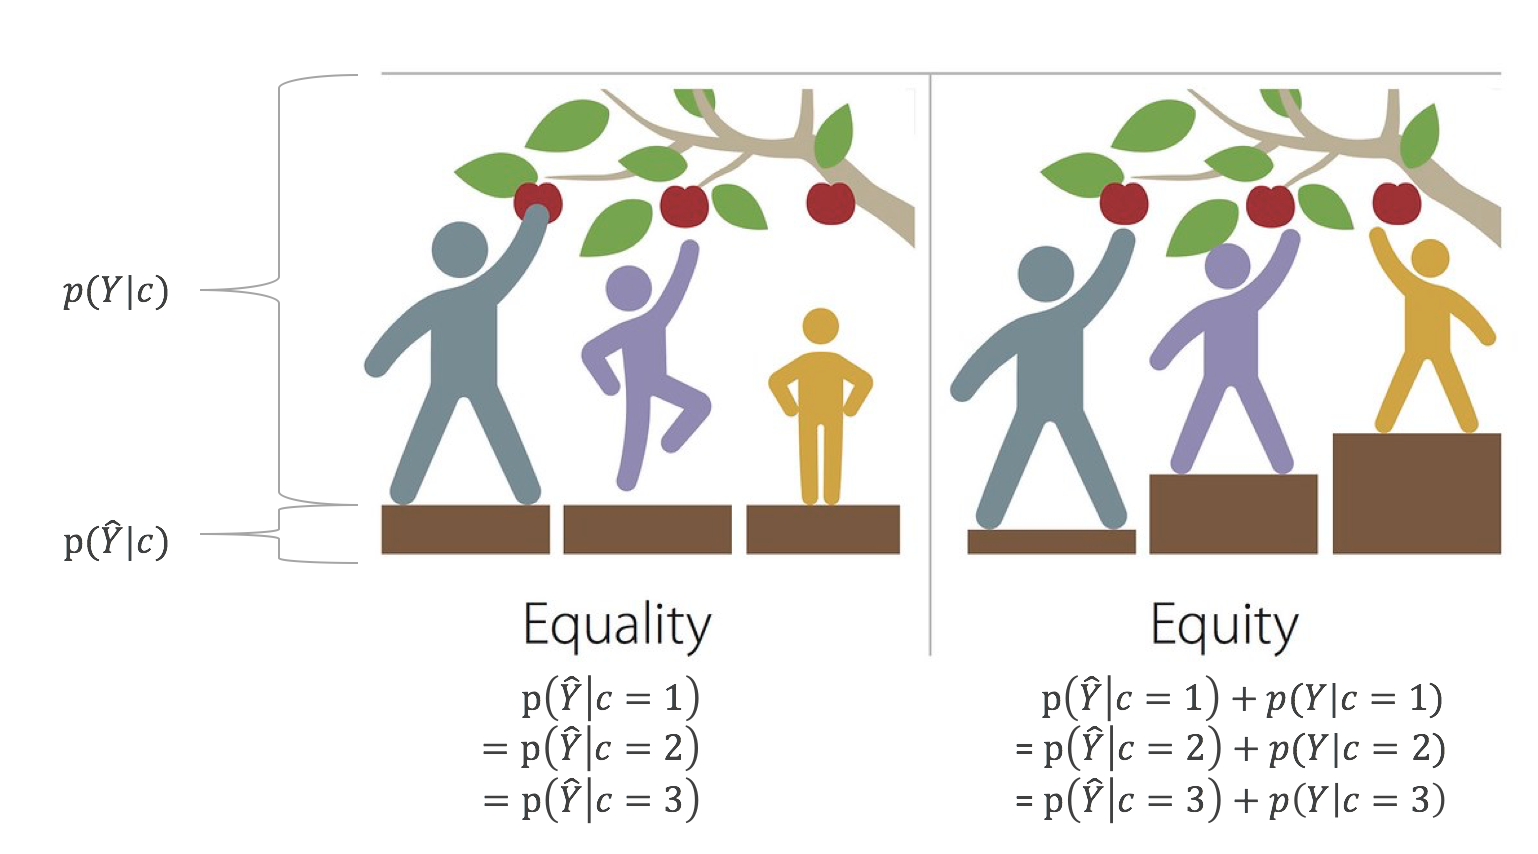
\includegraphics[width=0.5\textwidth,height=0.3\textwidth,trim=1.0cm 0.5cm 0.5cm 0.5cm,clip=true]{./images/equity.png}
\hspace{-1em}
\begin{tikzpicture}
\node[inner sep=0pt] (image) at (0,0) {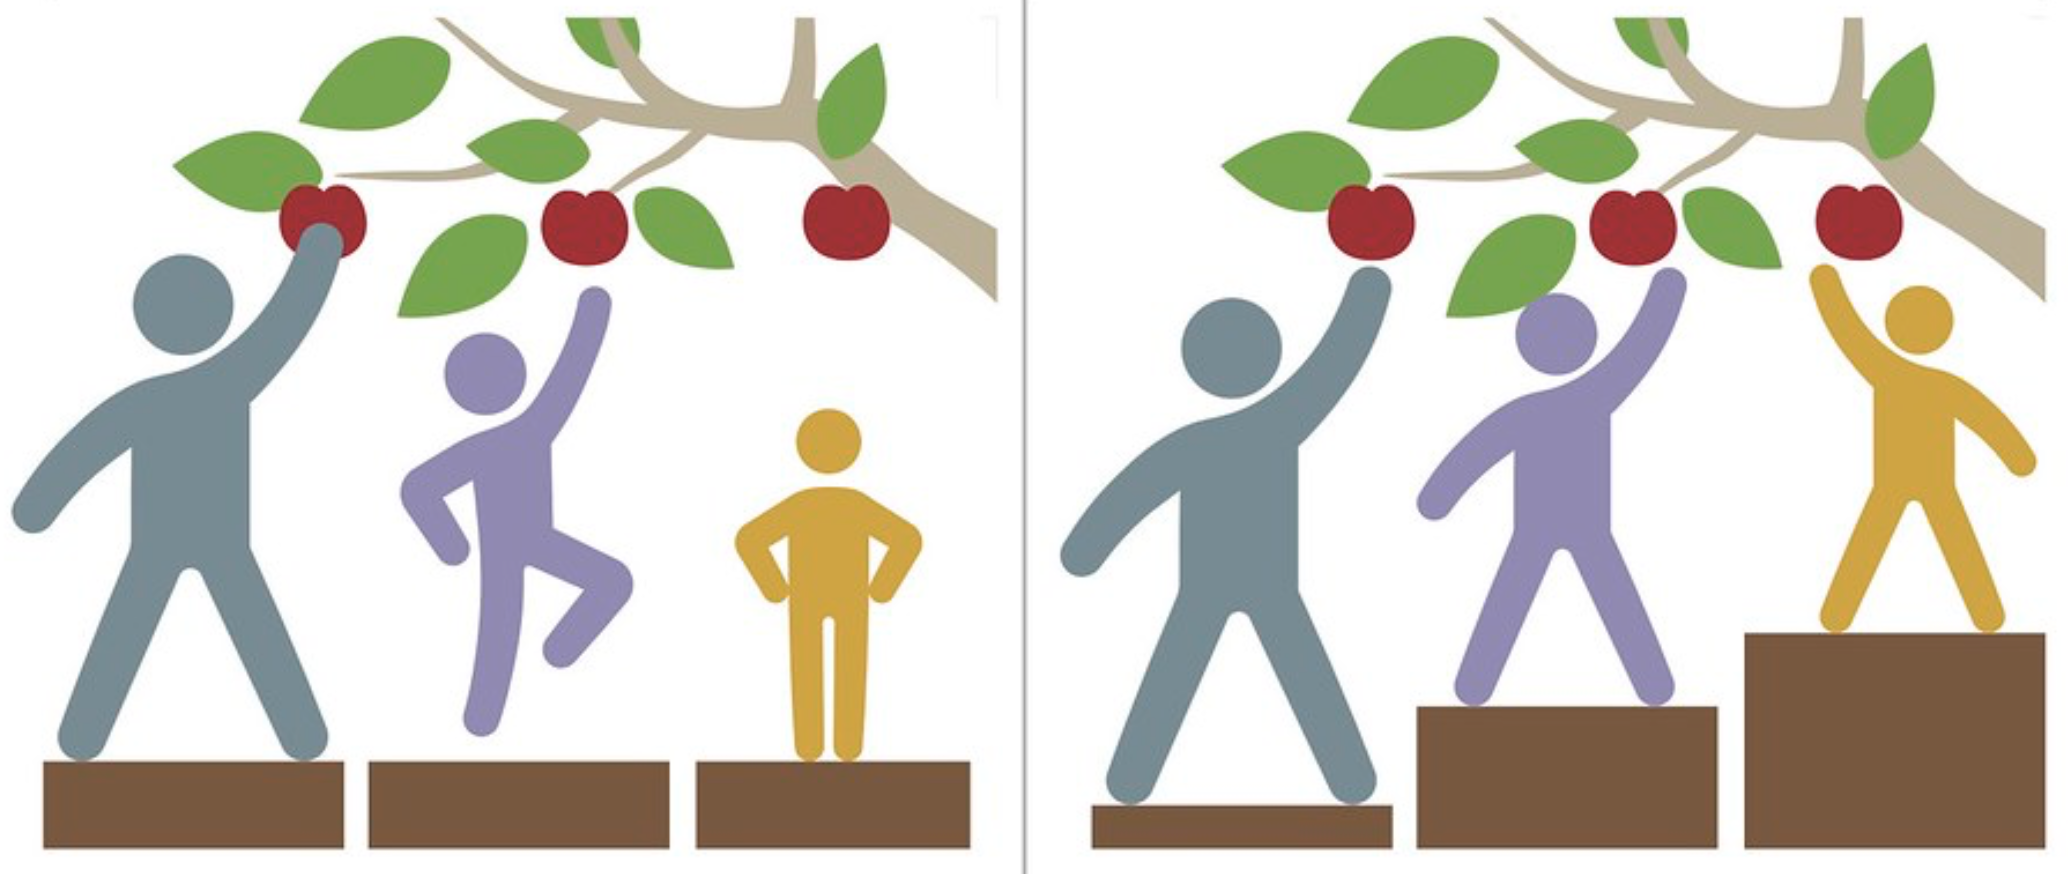
\includegraphics[width=0.85\columnwidth]{images/equity_without_text.png}};

\draw (-1.9, -1.8) node {Equality};
\draw (+1.5, -1.8) node {Equity};

\scriptsize
\draw (-2.4, -2.3) node {$p(\widehat{Y} | A=\text{blue})$};
\draw (-2.4, -2.7) node {$=p(\widehat{Y} | A=\text{purple})$};
\draw (-2.4, -3.1) node {$=p(\widehat{Y} | A=\text{yellow})$};

\draw (+1.6, -2.3) node {$p(\widehat{Y} | A=\text{blue}) + p(Y | A=\text{blue})$};
\draw (+1.6, -2.7) node {$=p(\widehat{Y} | A=\text{purple}) + p(Y | A=\text{purple})$};
\draw (+1.6, -3.1) node {$=p(\widehat{Y} | A=\text{yellow}) + p(Y | A=\text{yellow})$};

\draw [pen colour={black!50},decorate,decoration={brace,amplitude=6pt}]
(-3.4,-1.1) -- (-3.4,+0.65) node [black] {};
\draw [pen colour={black!50},decorate,decoration={brace,amplitude=4pt}]
(-3.4,-1.4) -- (-3.4,-1.12) node [black] {};

\draw (-4.1, -0.225) node {$p(Y|A)$};
\draw (-4.05, -1.275) node {$p(\widehat{Y}|A)$};

\end{tikzpicture}
% 
\includegraphics[width=0.5\textwidth,height=0.3\textwidth,trim=2.0cm 1.0cm 5.0cm 5.5cm,clip=true]{./images/motivation.pdf}
\caption{Notion of equality in fairness is depicted and formalized along with our newly formalized notion of equity.}
\label{motivation}
\end{figure}
 In light of that, we propose and mathematically formalize the equity notion of fairness in which resources and outcomes are distributed to overcome obstacles experienced by groups in order to maximize their opportunities \cite{schement2001imagining}. In this work we take the perspective that historical biases should be compensated and disadvantaged groups should be leveraged. We then introduce a data-driven classification objective function that operationalizes the notion of equity in which existing historical biases in the training data are compensated through predictions on the test data. 
 %One sentence about ``how''
 %This objective leverages historically disadvantaged groups with consideration to the needs of other demographic groups. 
 This approach will not only target fixing biases but it will also target minimizing the feedback loop phenomenon in which the biased data contaminates the decision making outcome, and it continues to stay and grow through the system. 
 
Our definition of fairness is an augmented version of statistical parity~\cite{Dwork:2012:FTA:2090236.2090255} that we adapt to measure equity. Unlike previous definitions and objective functions in which only equality is considered in present outcomes, our approach will consider the historical biases present in the data and will combine the notion of equity and affirmative action while also satisfying equality amongst groups. Our definition is a departure from differential privacy \cite{jagielski2019differentially} and fairness through unawareness \cite{10.1145/3287560.3287594} since having access to sensitive attributes is necessary in some scenarios. For instance, in cases that pertain to the medical domain, access to sensitive attributes such as gender and age are required to make a decision.

Two different fairness realizations are depicted in Figure \ref{motivation}. On the left side there is the notion of equality in which every group is given an equal amount of resources, which is too much for some members and insufficient for others. This is the problem that motivates this work: how can a classifier produce predictions that are good for the majority of a group or society? This leads us to the right picture which depicts equity where leverage is given through the model to give the groups appropriate resources to reach their goals. \\
%On the right, there is the notion of equity in which some groups are given more leverage to reach their goals, while on the left hand side there is the notion of equality in which every group is given an equal amount of leverage. Here, we model the required leverage given to each group as the outcome of the prediction $p(\hat{Y}|A)$ in the test set, while the height of people in the picture as $p(Y|A)$ representing the existing and historical biases in the training data. Here A indicates the belonging demographic group of each individual. Thus, according to the statistical parity notion the equality among groups $a$ and $b$ gets formalized as $p(\hat{Y}|A=a)=p(\hat{Y}|A=b)$, while we formalize the notion of equity among groups $a$ and $b$ as $p(\hat{Y}|A=a)+p(Y|A=b)=p(\hat{Y}|A=a)+p(Y|A=b)$.
\textbf{Note}: We use parity (statistical parity) and equality interchangeably as synonyms throughout this paper. \\ \\
The contributions of this paper are as follows:
\begin{enumerate}
    \item We define and formalize equity as a fairness definition.
    % \item Second, we couple this definition with the cross-entropy loss into the objective of our classification task and through experimentation show how it compares to the objective of equality.
    \item We demonstrate how this definition can be made actionable by proposing a loss function that combines equity with the cross-entropy loss into the classifier.
    Through experimentation, we demonstrate how our definition compares to the objective of equality.
    \item We then discuss and experimentally show the effectiveness of our definition in mitigating the feedback loop problem \cite{chouldechova2018frontiers}.
    \item Finally, we evaluate our fairness notion against the parity notion through human annotators and show how these definitions fare in different real life scenarios.
\end{enumerate}
